\section{Szerkesztő}
\rhead{Szerkesztő}

\subsection{A szerkesztő célja}

Az Archytex szerkesztő célja egy eszköz biztosítása építészeti látványtervek elkészítésére. A kész
jelenetek a beépített \emph{renderelés} funckió segítségével élethű képekké, professzionális
építészeti vizualizációkká alakíthatók, amelyek használhatók hobbi szinten, portfólió építésére vagy
akár professzionális munkához.

\subsection{Térbeli navigáció}

A szerkesztő legalapvetőbb eszköze a mozgatható kamera, hisz nélküle egy másik eszközt sem lehet
hasznosan alkalmazni. Szerencsére működése nagyon egyszerűen elsajátítható. Ahhoz, hogy a kamera
mozogjon, nyomva kell tartani a \emph{jobb egérgombot} egészen addig, amíg mozogni szeretnénk.
A \emph{jobb egérgomb} elengedésekor a kamera kilép a mozgó üzemmódból. Miközben a kamera mozgó
üzemmódban van, előre, hátra, balra és jobbra a \emph{W, S, A és D}, míg le és
fel az \emph{E és Q} billentyűkkel mozog. A kamera célirányának változtatása az egér mozgatásával
érhető el.

\subsection{Általános műveletek}

Létezik több olyan művelet, ami annyira általános, hogy bármilyen kontextusból elérhető.

\subsubsection{Visszavonás}

Bármilyen műveletet vissza lehet vonni a \emph{Ctrl+Z} billentyűkombinációval. Ilyenkor a
szerkesztő eltárolja a visszavont műveletet, hogy azt később meg lehessen ismételni. Ha az eltárolt
műveletek mennyisége eléri a hatvannégyet, a legrégebbi törlésre kerül.

\subsubsection{Ismétlés}

Ha a visszavont műveletek listája nem üres, akkor a \emph{Ctrl+Y} billentyűkombinációval kiadott
\emph{ismétlés} művelet megismétli a legújabban visszavont műveletet.

\pagebreak

\subsubsection{A rács nagyítása és kicsinyítése}

A szerkesztőben minden elem pozíciója egy négyzetes rácshoz igazodik. Az alapértelmezett rács
oldalhossza \emph{1 méter}, viszont gyakran előfordul, hogy ez túl nagy, vagy éppen túl kicsi.
Ilyenkor az \emph{O} billentyű lenyomásával a rács oldalhossza felére csökken, míg a \emph{P}
billentyű lenyomásával kétszeresére nő.

\begin{figure}[h]
    \centering
    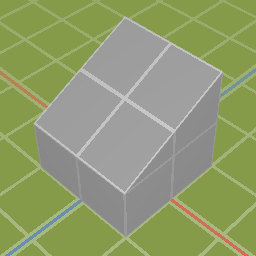
\includegraphics[width=0.25\textwidth]{parts/user-documentation/editor/images/grid_128.png}
    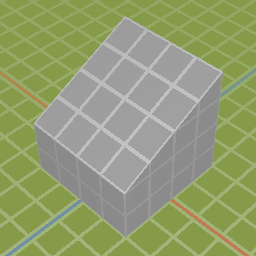
\includegraphics[width=0.25\textwidth]{parts/user-documentation/editor/images/grid_64.png}
    \caption{Azonos alakzat különböző rács oldalhosszúsággal}
\end{figure}

\subsubsection{Kijelölés}

A jelenet bármely eleme kijelölhető. Egy elem kijelöléséhez két feltételnek kell teljesülnie: az
\emph{egérmutatónak} az elem felett kell lennie, és meg kell nyomni a \emph{bal egérgombot}. Ha ez
úgy történik meg, hogy már léteznek kijelölt elemek, akkor azok a kijelölések megszűnnek. Ha az
előző kijelölés \emph{bővítése} a cél, akkor a \emph{Shift} billentyűt is nyomva kell tartani.
Érdemes megjegyezni, hogy ha ilyenkor rákattintunk egy kijelölt elemre, az a kijelölés megszűnik,
viszont a többi megmarad.

\begin{figure}[h]
    \centering
    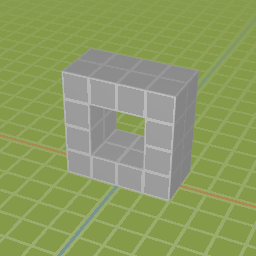
\includegraphics[width=0.25\textwidth]{parts/user-documentation/editor/images/unselected.png}
    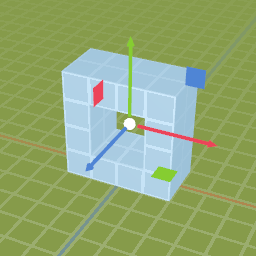
\includegraphics[width=0.25\textwidth]{parts/user-documentation/editor/images/selected.png}
    \caption{Azonos alakzat alapállapotban és kijelölve}
\end{figure}

\subsubsection{Mozgatás}

A jelenet bármely kijelölt eleme mozgatható. Olyan esetben, amikor a mozgatás engedélyezett,
látható a képernyőn a \emph{speciális mozgatóeszköz}. Az eszköz három színezett nyílból és három
színezett négyzetből áll.

\begin{figure}[h]
    \centering
    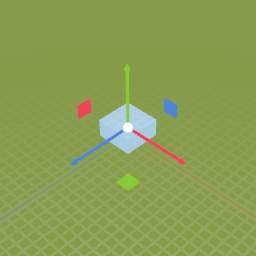
\includegraphics[width=0.25\textwidth]{parts/user-documentation/editor/images/move_gizmo.png}
    \caption{Speciális mozgatóeszköz}
\end{figure}

A nyilak a tér három tengelye, míg a négyzetek a tér három síkja mentén
mozgatják a kijelölt elemeket. Használathoz egyszerűen \emph{rá kell kattintani} a nyílra vagy
négyzetre. Az elemek abba az irányba fognak elmozdulni, amerre az \emph{egérmutató} mozog. A
\emph{bal egérgombot} addig kell lenyomva tartani, amíg az elemek nem kerültek a megfelelő helyükre.

\begin{figure}[h]
    \centering
    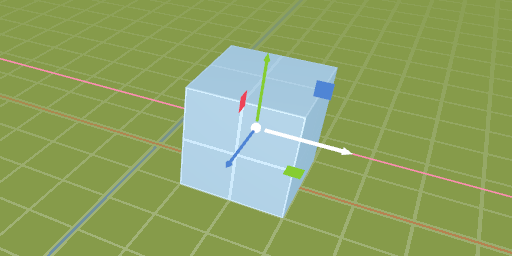
\includegraphics[width=0.5\textwidth]{parts/user-documentation/editor/images/move_in_action.png}
    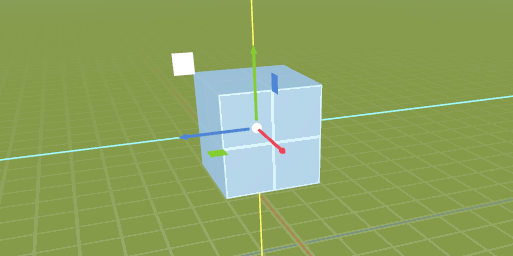
\includegraphics[width=0.5\textwidth]{parts/user-documentation/editor/images/move_in_action_plane.png}
    \caption{Elemek mozgatása a speciális mozgatóeszközzel}
\end{figure}

\subsubsection{Gyors mozgatás}

A kijelölt elemeket nem csak a \emph{speciális mozgatóeszköz} segítségével lehet mozgatni. Létezik
egy ún. \emph{gyors mozgatás} eszköz is, amit teljes mértékben billentyűkombinációk és egérmozgatás
vezérel. A \emph{gyors mozgatás} aktiválásához meg kell nyomni a \emph{G} billentyűt. Miután ez
megtörtént, ki kell választani, hogy melyik tengely vagy sík mentén mozogjanak az elemek. Az
\emph{X, Y vagy Z} billentyű lenyomása kiválasztja a hozzátartozó tengelyt. Sík kiválasztása is
hasonló módon történik: a \emph{Shift} billentyű lenyomása közben az \emph{X, Y, vagy Z} billentyű
a \emph{hozzátartozó tengelyre merőleges} síkot választja ki. Kiválasztás után az elemek az
\emph{egérmutatóval} mozognak. Ha az elemek elérték a megfelelő pozíciót, a \emph{bal egérgomb}
lenyomásával befejezhető a művelet. Abban az esetben, ha kiderül, hogy a mozgatás mégsem célszerű,
a \emph{G} billentyű, az \emph{Escape} billentyű, vagy a \emph{jobb egérgomb} lenyomásával megszakítható a mozgatás.

\subsection{Test szerkesztési mód}

Az általános műveletek mellett a szerkesztő támogat ún. \emph{speciális műveleteket} is, amik csak
bizonyos \emph{módokban} használhatók. A szerkesztőnek négy különböző \emph{módja} van, ezek közül
az első -- és egyben alapértelmezett -- a \emph{test szerkesztési mód}. Az Archytex jelenetek
kétféle elemet tartalmazhatnak: \emph{testeket} és \emph{díszítőelemeket}. A
\emph{test szerkesztési mód} magától értetődően a \emph{testek} kezelését, manipulációját teszi
lehetővé.

\subsubsection{Létrehozás}

Új \emph{test} létrehozásához nyomva kell tartani a \emph{bal egérgombot}. Miközben ez történik, az
\emph{egérmutató} mozgatásával módosítható a létrejövő \emph{test} mérete. A \emph{bal egérgomb}
elengedésekor az új \emph{test} véglegessé válik.

\subsubsection{Törlés}

Egy vagy több kijelölt \emph{test} törölhető a \emph{Delete} billentyű lenyomásával.

\pagebreak

\subsubsection{Forgatás}

Gyakran előfordulhat, hogy szimmetrikus alakzatok elkészítésére van szükség. Ilyenkor jól jöhet a
\emph{test forgatása} eszköz, amely segítségével a kijelölt \emph{testeket} bármely bázis tengely
körül lehet forgatni $90^{\circ}$-os vagy $-90^{\circ}$-os szöggel.

\begin{figure}[h]
    \centering
    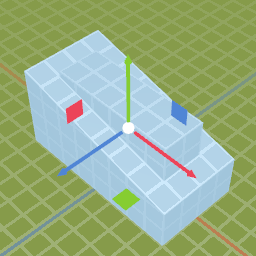
\includegraphics[width=0.25\textwidth]{parts/user-documentation/editor/images/rot1.png}
    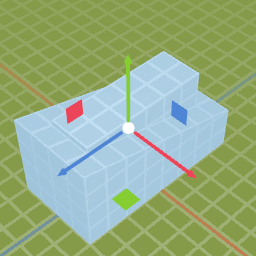
\includegraphics[width=0.25\textwidth]{parts/user-documentation/editor/images/rot2.png}
    \caption{Alakzat forgatás előtt és után}
\end{figure}

Az eszköz használatához jelöljön ki néhány \emph{testet}, majd nyomja le az \emph{F} billentyűt.
Miután ez megtörtént, válassza ki a megfelelő forgástengelyt az \emph{X, Y vagy Z} billentyű
lenyomásával. A forgástengely kiválasztása után a kijelölt \emph{testek} azonnal elfordulnak.
Ha a forgástengely kiválasztása közben a \emph{Shift} billentyű nincs lenyomva, a forgás szöge
$90^{\circ}$, ellenkező esetben $-90^{\circ}$.

\subsubsection{Üregesítés}

Bármely \emph{testet} azonnal üregessé lehet tenni a \emph{H} billentyű lenyomásával. Ez a művelet
főleg beltéri területek kialakítására hasznos. Az új, üreges tér falainak vastagságát a \emph{rács}
oldalhossza adja meg.

\begin{figure}[h]
    \centering
    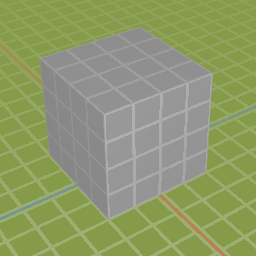
\includegraphics[width=0.25\textwidth]{parts/user-documentation/editor/images/hollow1.png}
    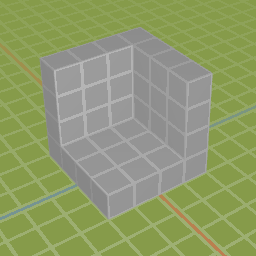
\includegraphics[width=0.25\textwidth]{parts/user-documentation/editor/images/hollow2.png}
    \caption{Test üregesítés előtt és után (néhány fal láthatatlan a példa kedvéért)}
\end{figure}

\subsubsection{Másolás}

Egy vagy több kijelölt \emph{test} másolásához nyomja le a \emph{C} billentyűt. Ilyenkor a
szerkesztő \emph{gyors mozgatás} üzemmódba lép, így a lemásolt \emph{testek} azonnal mozgathatóvá
válnak.

\begin{figure}[h]
    \centering
    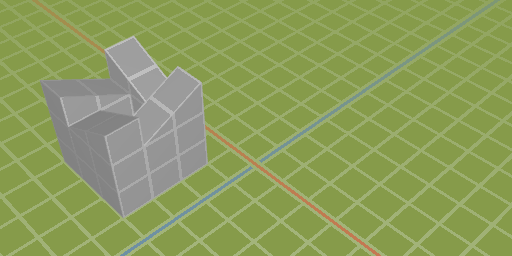
\includegraphics[width=0.5\textwidth]{parts/user-documentation/editor/images/copy1.png}
    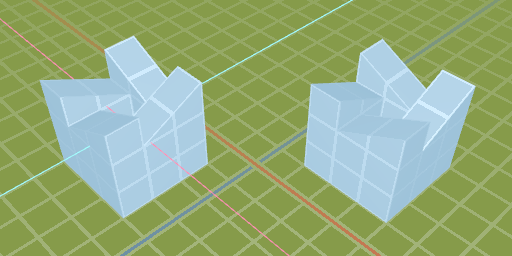
\includegraphics[width=0.5\textwidth]{parts/user-documentation/editor/images/copy2.png}
    \caption{Testek másolása}
\end{figure}

\subsection{Lap szerkeszési mód}

\subsubsection{Textúrázás}

A \emph{lap szerkesztési mód} egyetlen \emph{speciális művelete} a \emph{textúrázás}. Válassza ki a használni kívánt \emph{textúrát} a \emph{textúra könyvtárból}, majd jelöljön ki egy vagy több
\emph{lapot}, és nyomja le a \emph{T} billentyűt. A kijelölt \emph{lapokon} ezentúl a kiválasztott
\emph{textúra} fog megjelenni.

\begin{figure}[h]
    \centering
    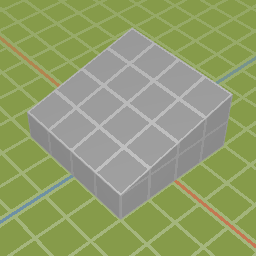
\includegraphics[width=0.25\textwidth]{parts/user-documentation/editor/images/tex1.png}
    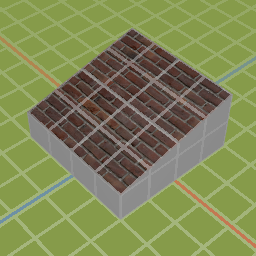
\includegraphics[width=0.25\textwidth]{parts/user-documentation/editor/images/tex2.png}
    \caption{Lap textúrázás előtt és után}
\end{figure}

\pagebreak

\subsection{Csúcs szerkesztési mód}

Mivel egy \emph{csúcs} egyetlen tulajdonsága a térbeli elhelyezkedése, ezért a
\emph{csúcs szerkesztési mód} nem tartalmaz további \emph{speciális műveletet.}

\begin{figure}[h]
    \centering
    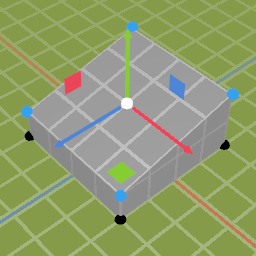
\includegraphics[width=0.25\textwidth]{parts/user-documentation/editor/images/vertices.png}
    \caption{Csúcsok mozgatása}
\end{figure}

\subsection{Berendező mód}

A szerkesztő negyedik, és egyben utolsó \emph{módja} a különböző \emph{díszítőelemek} kezelését és
manipulációját teszi lehetővé.

\subsubsection{Forgatás}

A \emph{testekkel} ellentétben a \emph{díszítőelemek} bármely tengely körül, bármilyen szöggel
elforgathatóak. Egy vagy több \emph{díszítőelem} kijelölése után megjelenik a
\emph{speciális forgatóeszköz}. Az eszköz három, egymásra merőleges színezett körből áll.
Forgatáshoz húzza az \emph{egérmutatót} a forgástengelyhez tartozó kör fölé, majd tartsa lenyomva
a \emph{bal egérgombot}. A kijelölt \emph{díszítőelemek} az \emph{egérmutató} mozgása szerint
fognak forogni.

\begin{figure}[h]
    \centering
    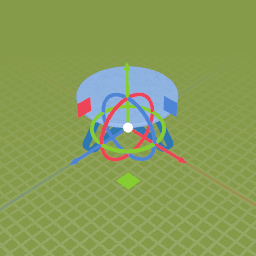
\includegraphics[width=0.25\textwidth]{parts/user-documentation/editor/images/rotate_gizmo.png}
    \caption{Speciális forgatóeszköz}
\end{figure}

\subsubsection{Gyors forgatás}

A kijelölt \emph{díszítőelemeket} nem csak a \emph{speciális forgatóeszköz} segítségével lehet
forgatni. Ebben a \emph{módban} az általános \emph{gyors mozgatás} mellett létezik a
\emph{gyors forgatás} művelet is. A művelet megkezdéséhez nyomja le az \emph{R} billentyűt.
A forgatás csak a forgástenglely kiválasztása után lehetséges. Ez
az \emph{X, Y vagy Z} billentyű lenyomásával tehető meg. Miután ez megtörtént, a kijelölt
\emph{díszítőelemek} az \emph{egérmutató} mozgása szerint forognak. A \emph{Ctrl} billentyű
nyomvatartása a forgás szögét $15^{\circ}$-os lépésekre korlátozza.

\subsubsection{Forgás alapállapotba állítása}

Az \emph{R} billentyű kétszeri lenyomásával a kijelölt \emph{díszítőelemek} forgása visszaáll
alapállapotba.

\subsubsection{Másolás}

A \emph{díszítőelemek} másolása teljesen úgy működik, mint a \emph{testek} másolása.

\subsection{Mentés és renderelés}

Az Archytex szolgáltatás ingyen tárhelyet biztosít a jeleneteknek és a képeknek. Az épp betöltött
jelenet mentéséhez nyomja meg a \emph{Mentés} gombot.

A kész jelenetekről könnyedén lehet élethű képeket készíteni. Nyomja meg a \emph{Renderelés} gombot,
és állítsa be a megfelelő paramétereket a felugró ablakban. Miután mindent beállított, nyomja meg
a \emph{Render indítása} gombot. Ezután akár el is hagyhatja az oldalt, mivel a kirajzolás
folyamata a háttérben, az Archytex szerverein fog megtörténni. A kész képeket a \emph{Vezérlőpultban} a projektre kattintás után tekintheti
meg.

\begin{figure}[h]
    \centering
    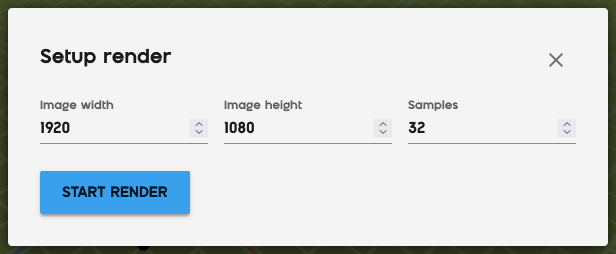
\includegraphics[width=0.5\textwidth]{parts/user-documentation/editor/images/render.png}
    \caption{Render beállítások}
\end{figure}